% previousresearch.tex

% Previous Research
\section{Previous Research and Background}
\label{sec:previousresearch}
System simulators are abundant and exist in corporate~\masccitebib{magazines:bohrer:2004}, academic~\masccitebib{journals:rosenblum:1995}, and open-source variations~\mascciteref{inproceedings:bellard:2005}.
Such platforms, like Simics, are used for many purposes including thermal control strategies in multicores~\masccitebib{inproceedings:bartolini:2010}, networking timing analysis~\masccitebib{journals:ortiz:2009}, web server performance evaluation~\masccitebib{journals:villa:2005}, and to simulate costly hardware financially unfeasible to researchers~\masccitebib{journals:alameldeen:2003}.

QEMU ('Quick~Emulator') is an open-source virtual platform described as a full system emulator~\masccitebib[p.~1]{inproceedings:bellard:2005} and a high-speed functional simulator~\masccitebib[p.~1]{inproceedings:shen:2010}.
As such, QEMU may run unmodified target software such as OSs, drivers, and other applications~\masccitebib[p.~1]{inproceedings:bellard:2005}.
The platform is widely used in academia, and is the subject of several articles and reports cited throughout this document.

Several attempts have been made to accelerate simulator graphics.
Many of these require modification of both target and host systems.
One such instance is presented by Hansen in his work on the Blink display system~\masccitebib{inproceedings:hansen:2007}.
Another example, the Android emulator, which is powered by QEMU, accelerates OpenGL~ES~$1.1$ and $2.0$, granting Android developers significant performance boosts~\mascciteref{web:ducrohet:2012:afasteremulator}.

Lagar-Cavilla et al. present VMGL, an OpenGL virtualization solution that can accelerate OpenGL~$1.5$ up to two orders of magnitude in comparison to software rasterization~\masccitebib{inproceedings:lagarcavilla:2007}.
The solution runs the OpenGL library and GPU driver on the VMM host, and utilizes network transport to relieve OpenGL commands between target and host systems.
VMGL was evaluated in WMware Workstation and Xen VMMs.

Other related works include modeling GPU devices in the QEMU full-system simulator with software OpenGL~ES rasterization support, as presented by Shen et al.~\masccitebib{inproceedings:shen:2010}.
Current promising GPU virtualization projects include the Virgil3D-project~\mascciteref{technicaldocs:qemudevel:2014}.
The project strives to create a virtual GPU which may utilize host hardware to accelerate 3D rendering.

% Simics
\subsection{Simics}
\label{sec:simics}
Simics is a full-system simulator developed by Intel and sold through Intel's subsidiary Wind~River~Systems.
Simics was originally developed at the Swedish Institute of Computer Science~\masccitebib{inproceedings:werner:1997}, commercially launched by Virtutech in $1998$~\masccitebib{publications:leupers:2010}, and subsequently acquired by Intel in $2010$~\masccitebib{journals:aarno:2013}.

As an architectural simulator, Simics' primary client group is software and systems developers that produce software involving software and hardware interaction~\masccitebib{journals:aarno:2013}.
The simulator utilizes hardware-assisted virtualization and other performance boosting technologies such as hyper-simulation~\masccitebib[p.~38]{publications:leupers:2010} to accelerate simulation speeds.
Simics also feature advanced functionality adhering to the deterministic nature of the simulator, such as checkpointing and reverse execution~\masccitebib{journals:aarno:2013, publications:aarno:2014}.

The ability to simulate an unmodified software stack has led to Simics being used to simulate a variety of systems including single-processor embedded boards, multiprocessor servers, and heterogeneous telecom clusters~\masccitebib{journals:aarno:2013}.
Employers of Simics include Intel~\masccitebib{publications:aarno:2014, misc:moestedt:2015}, NASA~\masccitebib{publications:aarno:2014, misc:moestedt:2015}, and Lockheed Martin~\mascciteref{misc:moestedt:2015}.
Furthermore, the simulator has a strong academic tradition -- known to operate in over $300$ universities~\masccitebib[p.~252]{journals:villa:2005}.

% Graphics Virtualization
\subsection{Graphics Virtualization}
\label{sec:previousresearch_graphicsvirtualization}
There are a number of ways of virtualizing GPUs in virtual platforms, a few of which accommodate hardware acceleration; fewer that suit most needs.
Therefore, it is important to balance desired simulation level of detail with performance requirements.
As such, virtualization methods with varying simulation accuracy present themselves, from slow low level instruction set modeling to fast high level paravirtualization.
Summaries of some viable strategies are presented below.

% GPU Modeling
\paragraph{GPU Modeling}
\label{par:previousresearch_graphicsvirtualization_gpumodeling}
Some may consider virtualizing the GPU ISA.
This could be appropriate for the purposes of development close to GPU hardware.
For example, one might imagine the scenario of driver development for next-generation GPUs.

However, the development of a GPU model might be overly costly, due to GPU hardware being poorly documented compared to CPU architectures~\masccitebib{inproceedings:lagarcavilla:2007}.
Furthermore, simulating massively parallelized GPU ISAs induce high performance costs that might render GPU modeling less preferable for development requiring anything but slow simulation speed.

% PCI Passthrough
\paragraph{PCI Passthrough}
\label{par:previousresearch_graphicsvirtualization_pcipassthrough}
PCI~passthrough technologies allow virtual systems first-hand access to host machine devices~\mascciteref{inproceedings:regola:2010}, accommodating for fully-fledged hardware accelerated workloads.
However, this requires \textit{dedicated} hardware on host systems and requires configuring the simulation target to utilize host hardware.
For example, this may induce the necessity of multiple graphics cards on the host system.
Furthermore, PCI~passthrough is likely to make it difficult to implement robust checkpointing and reverse execution functionality, should advanced simulation features be desirable.

% Paravirtualization
\paragraph{Paravirtualization}
\label{par:previousresearch_graphicsvirtualization_paravirtualization}
At a higher level of abstraction, there is the option of paravirtualization.
By selectively modifying the target system, it is possible to control system attributes and add functionality such as device hardware support, and advanced functionality such as checkpointing and reverse execution may be facilitated in software.
For graphics acceleration, such a system attribute could be a graphics library or a kernel driver (see Figure \ref{fig:overview}).

Inherent by higher abstraction, paravirtualization is cheap in terms of development costs, and by selectively modifying at the graphics library level, there is no need for users to modify the software they wish to accelerate.
Unfortunately, a paravirtualized graphics library may be troublesome to maintain as the framework evolves.
Furthermore, it requires modification of the simulation target, which may be undesirable for some.
Optimally, the simulator should run an unmodified target, but if high performance is important enough for compromise, paravirtualization at the graphics library level is a good trade-off to delimit required modification.
In this way, the changes are confined to the graphics library.
Thus, what parts of the simulation are modified can easily be described to systems developers.

\begin{figure}
\centering
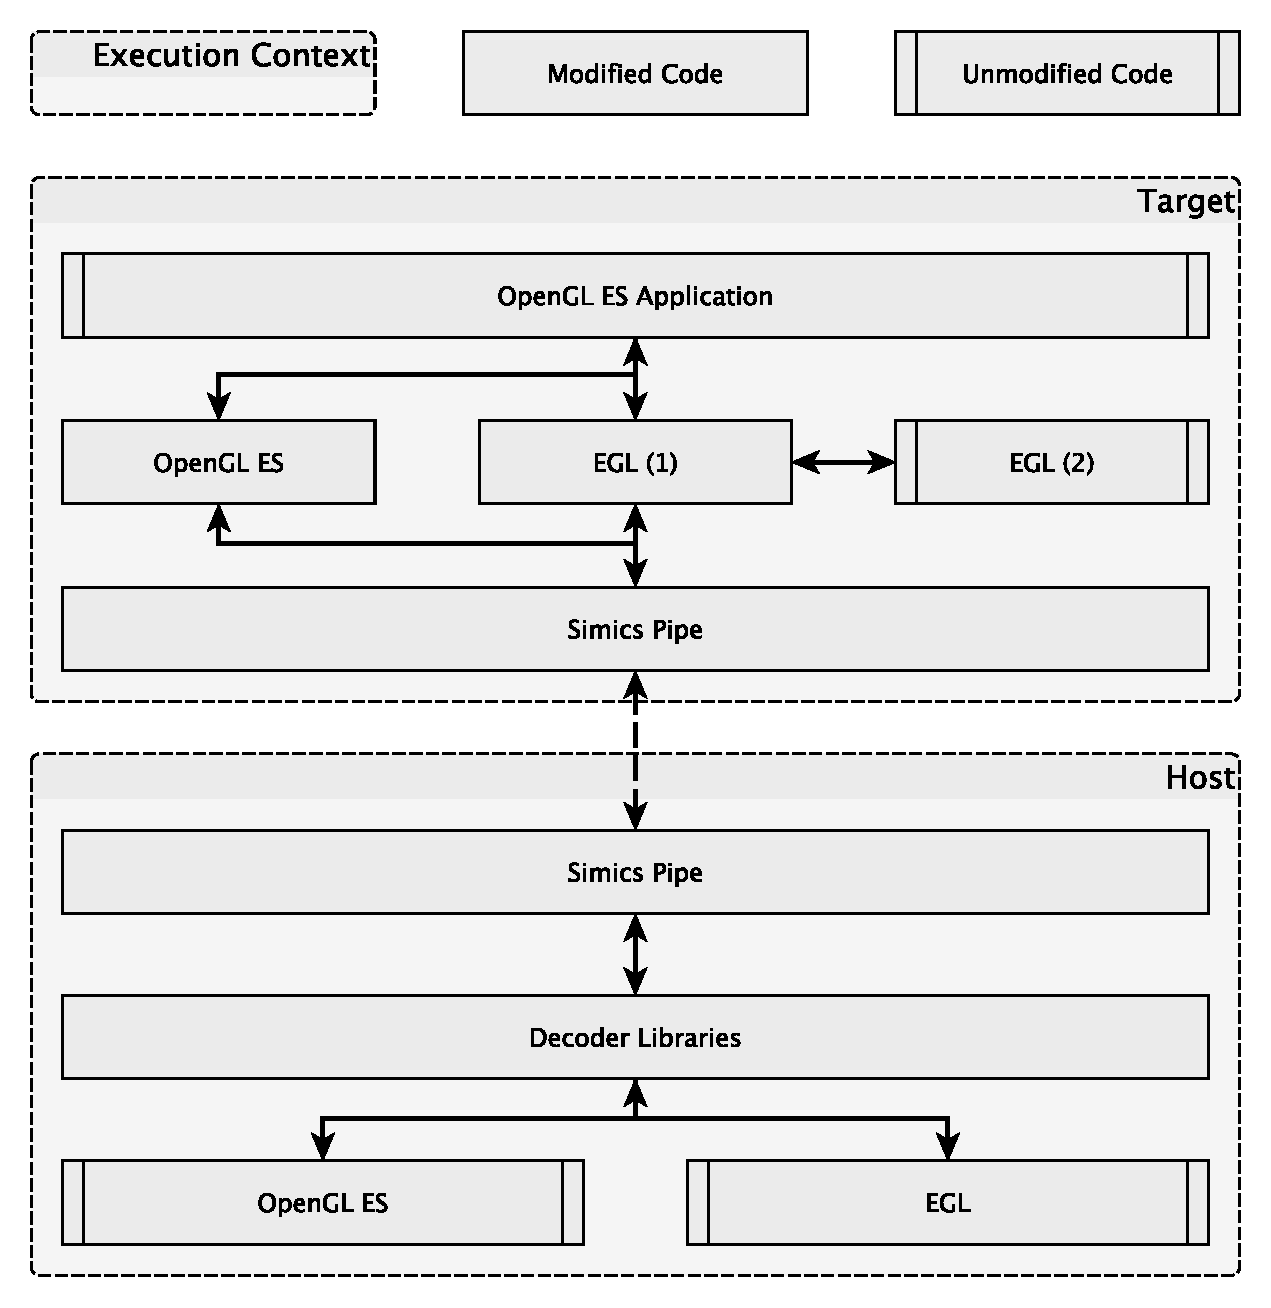
\includegraphics[width=\linewidth]{img/yedoverview.pdf}
\caption{Overview of paravirtualized graphics in Simics.}
\label{fig:overview}
\end{figure}
